\pagebreak
\subsection{Thermal Design} \label{Thermal_section}

\subsubsection{Thermal Environment}
\begin{centering}
The experiment will experience a wide range of temperatures during the flight and it must be able to continue to operate despite these changes. As seen in Figure \ref{fig:temperature-profile} the coldest point of the flight will be between 10km and 15km where the air temperature can drop to $-80\degree$C and temperatures on the gondola have been recorded as low as $-40\degree$C during the float phase in the past \cite{BexusManual}. In addition launching from Kiruna in late October means the temperature on the ground could be as low as $-10\degree$C. 
%The lowest operating temperature is 5 so can be lower before.
As our lowest operating temperature component must be at a minimum of $5\degree$C this could mean heaters will need to be switched on while the experiment is still on the ground. 
\end{centering}


\begin{figure}[H]
    \begin{align*}
        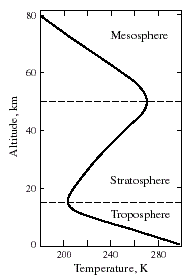
\includegraphics[height=5cm]{4-experiment-design/img/temperature-profile.png}
    \end{align*}
    \caption{Diagram showing the temperature profile of the atmosphere \cite{jacob}}\label{fig:temperature-profile}
\end{figure}

\subsubsection{Overall Design}
\begin{centering}
To protect the components against the cold two heaters will be included. One of these will be placed close to the pump to keep it warm when it is not active. The second and third heaters will be placed adjacent to the valve manifold to ensure the valves continue to operate as expected. To control these heaters two temperature sensors will also be onboard in similar locations. If the reading from one of the temperature sensors is lower than the predefined threshold then the heater will turn on. 
\end{centering}

% New for the SED v2
The main protection against the cold environment in the stratosphere is a passive thermal design, it is for this case thermal insulation. It will be two layers, one outer sheet of aluminum and a thicker sheet of styrofoam. The main insulating factor is the styrofoam and it will be 20mm of styrofoam. \\
There will also be a active thermal control consisting off three heaters. One will be attached to the pump. The other two will be attached to the two manifolds that the valves are connected to. The pump and valves are the most critical components. To determine the uniform heat inside MATLAB will be used. Then by using ANSYS to simulate the condition inside the brain box.
The heaters will be controlled by the Arduino with the help of temperature sensors. If the temperature is beneath a certain level the heaters will turn on to get the pump or the valve to their required temperature.
%

\begin{centering}
In addition to using electrical heaters the experiment will also be thermally insulated. A layer of aluminum sheeting will cover the experiment's exterior to reflect a portion of solar radiation, and the Styrofoam casing which will be used to protect the CAC from impact forces will also serve as insulation. %It is also planned to add additional insulation around the components.  
\end{centering}



\pagebreak


%Added this space to help us see all of the numbers. This "Track changes" sign blocks them every time!


\begin{longtable}{|m{1cm}|m{3.5cm}|m{1.3cm}|m{1.3cm}|m{1.4cm}|m{1.3cm}|m{1.3cm}|m{1.3cm}|}
\hline
\multirow{2}{*}{\textbf{ID}} & \multirow{2}{*}{\textbf{Components}}                                 & \multicolumn{2}{l|}{\textbf{Operating (°C)}} & \multicolumn{2}{l|}{\textbf{Survivable (°C)}} & \multicolumn{2}{l|}{\textbf{Expected (°C)}} \\ \cline{3-8} &   & Min.  & Max.  & Min.  & Max.  &  Min.   &  Max.            \\ \hline
E1 & Arduino Due & -40 & 85 & -60 & 150 & -30.62 & 24.01 \\ \hline
E2 & Ethernet Shield & -40 & 85 & -65 & 150 & -30.62 & 24.01 \\ \hline
E3 & Miniature diaphragm air pump & 5 & 40 & -10 & 40 & 10 & 34.93 \\ \hline
E4 & Pressure Sensor & -40 & 85 & -40 & 125 & -19.70 & 34.93 \\ \hline
E5 & Sampling Valve (inlet and outlet 1/8"" female) & -20 & 50 & -20\footnote{If survivable temperatures were not given, operating temperatures were used as survivable limits.\label{fn:erik}} & 50\textsuperscript{\ref{fn:erik}} & -15 & 20 \\ \hline
E6 & Airflow sensor AWM43300V & -20 & 70 & -20\textsuperscript{\ref{fn:erik}} & 70\textsuperscript{\ref{fn:erik}} & -8.77 & 34.93 \\ \hline
E7 & Heater ($12.7\times 50.8 mm$) & -200 & 200 & -200\textsuperscript{\ref{fn:erik}} & 200\textsuperscript{\ref{fn:erik}} & -20 & 36 \\ \hline
E8 & Voltage Regulator & -40 & 125 & -40\textsuperscript{\ref{fn:erik}} & 125\textsuperscript{\ref{fn:erik}} & -30.62 & 34.93 \\ \hline
E9 & Temperature Sensor & -55 & 125 & -65 & 150 & -19.70 & 34.93 \\ \hline
E10 & DCDC 24 V & -40 & 85 & -55 & 125 & -19.70 & 34.93 \\ \hline
E12 & Micro SD & -25 & 85 & -200\textsuperscript{\ref{fn:erik}} & 200\textsuperscript{\ref{fn:erik}} & -19.70 & 34.93 \\ \hline
% E13 & Logic CAT5E & -20 & 75 & (-20)\textsuperscript{\ref{fn:erik}} & (75)\textsuperscript{\ref{fn:erik}} & TBD\textsuperscript{\ref{fn:ivan}} & TBD\textsuperscript{\ref{fn:ivan}} \\ \hline
% E14 & Resistors (33, 150 and 100 ohm) & -55 & 155 & (-55)\textsuperscript{\ref{fn:erik}} & (155)\textsuperscript{\ref{fn:erik}} & TBD\textsuperscript{\ref{fn:ivan}} & TBD\textsuperscript{\ref{fn:ivan}} \\ \hline
% E15 & Capacitors $(0.1 \mu$ F and $10 \mu$ F) & -30 & 85 & (-200)\textsuperscript{\ref{fn:erik}} & (200)\textsuperscript{\ref{fn:erik}} & TBD\textsuperscript{\ref{fn:ivan}} & TBD\textsuperscript{\ref{fn:ivan}} \\ \hline
E16 & Mosfet for current control & -55 & 175 & -55 & 175 & -20 & -20 \\ \hline
E17 & Diodes for DCDC converters & -65 & 175 & -65\textsuperscript{\ref{fn:erik}} & 175\textsuperscript{\ref{fn:erik}} & -19.70 & 34.93 \\ \hline
E18 & 3.3V LED & -40 & 85 & -40\textsuperscript{\ref{fn:erik}} & 85\textsuperscript{\ref{fn:erik}} & -19.70 & 24.01 \\ \hline 
E19 & 15-pin D-SUB Female connector with pins & -55 & 120 & -200\textsuperscript{\ref{fn:erik}} & 200\textsuperscript{\ref{fn:erik}} & -8.77 & 24.01 \\ \hline
E20 & 9-pin D-SUB Female connector with pins & -55 & 120  & -200\textsuperscript{\ref{fn:erik}} & 200\textsuperscript{\ref{fn:erik}} & -8.77 & 24.01 \\ \hline
E21 & 9-pin D-SUB Female connector with soldering cups & -55 & 105 & -55\textsuperscript{\ref{fn:erik}} & 105\textsuperscript{\ref{fn:erik}} & -8.77 & 24.01 \\ \hline
E22 & 9-pin D-SUB Male connector with soldering cups & -55 & 105 & -55\textsuperscript{\ref{fn:erik}} & 105\textsuperscript{\ref{fn:erik}} & -8.77 & 24.01 \\ \hline
E23 & 15-pin D-SUB Male connector with soldering cups & -55  & 105 & -55\textsuperscript{\ref{fn:erik}} & 105\textsuperscript{\ref{fn:erik}} & -8.77 & 24.01 \\ \hline
E24 & 9-pin D-SUB backing & -40 & 120 & -40\textsuperscript{\ref{fn:erik}} & 120 & -8.77 & 24.01  \\ \hline
E25 & 15-pin D-SUB backing & -40 & 120 & -40\textsuperscript{\ref{fn:erik}} & 120 & -8.77 & 24.01  \\ \hline
% E26 & Wall mounting bolts & TBD\textsuperscript{\ref{fn:ivan}} & TBD\textsuperscript{\ref{fn:ivan}} & TBD\textsuperscript{\ref{fn:ivan}} & TBD\textsuperscript{\ref{fn:ivan}} & TBD\textsuperscript{\ref{fn:ivan}} & TBD\textsuperscript{\ref{fn:ivan}} \\ \hline
E27 & D-SUB cable CAC to AAC & -40 & 85 & -55 & 125 & -40 & 40 \\ \hline
% E28 & 3.3 Zener diode & TBD\textsuperscript{\ref{fn:ivan}} & 175 & TBD\textsuperscript{\ref{fn:ivan}} & (175)\textsuperscript{\ref{fn:erik}} & TBD\textsuperscript{\ref{fn:ivan}} & TBD\textsuperscript{\ref{fn:ivan}} \\ \hline
E29 & Male connector on PCB & -40 & 85 & -40\textsuperscript{\ref{fn:erik}} & 85 & -8.77 & 24.01 \\ \hline
E30 & Female connector from wall & -40 & 85 & -40\textsuperscript{\ref{fn:erik}} & 85 & - & - \\ \hline
% E31 & Grounding contact & -55 & 125 & (-55)\textsuperscript{\ref{fn:erik}} & (125)\textsuperscript{\ref{fn:erik}} & TBD\textsuperscript{\ref{fn:ivan}} & TBD\textsuperscript{\ref{fn:ivan}} \\ \hline
E32 & Logic CAT5 E-link for inside box &-20 & 75 & -20\textsuperscript{\ref{fn:erik}} & 75\textsuperscript{\ref{fn:erik}} & -15 & 20 \\ \hline
E33 & Signal Wires & -60 & 200 & -60\textsuperscript{\ref{fn:erik}} & 200\textsuperscript{\ref{fn:erik}} & - & - \\ \hline
E34 & Flushing valve (inlet and outlet 1/8"" female) & -10 & 50 & -10\textsuperscript{\ref{fn:erik}} & 50\textsuperscript{\ref{fn:erik}} & -7.36 & 42.53 \\ \hline
E35 & Valves manifold (outlet 1/8"" female) & -10 & 50 & -10\textsuperscript{\ref{fn:erik}} & 50\textsuperscript{\ref{fn:erik}} & -6.77 & 40.504 \\ \hline
E36 & Power wire black & -60 & 200 & -60\textsuperscript{\ref{fn:erik}} & 200\textsuperscript{\ref{fn:erik}} & - & - \\ \hline
% E37 & Electrical Tape for marking wires (White) & -10 & 90 & (-10)\textsuperscript{\ref{fn:erik}} & (90)\textsuperscript{\ref{fn:erik}} & TBD\textsuperscript{\ref{fn:ivan}} & TBD\textsuperscript{\ref{fn:ivan}} \\ \hline
% E38 & Electrical Tape for marking wires (Black) & -10 & 90 & (-10)\textsuperscript{\ref{fn:erik}} & (90)\textsuperscript{\ref{fn:erik}} & TBD\textsuperscript{\ref{fn:ivan}} & TBD\textsuperscript{\ref{fn:ivan}} \\ \hline
% E39 & Electrical Tape for marking wires (Green) & -10 & 90 & (-10)\textsuperscript{\ref{fn:erik}} & (90)\textsuperscript{\ref{fn:erik}} & TBD\textsuperscript{\ref{fn:ivan}} & TBD\textsuperscript{\ref{fn:ivan}} \\ \hline
% E40 & Electrical Tape for marking wires (Violet) & -10 & 90 & (-10)\textsuperscript{\ref{fn:erik}} & (90)\textsuperscript{\ref{fn:erik}} & TBD\textsuperscript{\ref{fn:ivan}} & TBD\textsuperscript{\ref{fn:ivan}} \\ \hline
% E41 & Electrical Tape for marking wires (Gray) & -10 & 90 & (-10)\textsuperscript{\ref{fn:erik}} & (90)\textsuperscript{\ref{fn:erik}} & TBD\textsuperscript{\ref{fn:ivan}} & TBD\textsuperscript{\ref{fn:ivan}} \\ \hline
% E42 & Electrical Tape for marking wires (Brown) & -10 & 90 & (-10)\textsuperscript{\ref{fn:erik}} & (90)\textsuperscript{\ref{fn:erik}} & TBD\textsuperscript{\ref{fn:ivan}} & TBD\textsuperscript{\ref{fn:ivan}} \\ \hline
% E43 & Electrical Tape for marking wires (Blue) & -10 & 90 & (-10)\textsuperscript{\ref{fn:erik}} & (90)\textsuperscript{\ref{fn:erik}} & TBD\textsuperscript{\ref{fn:ivan}} & TBD\textsuperscript{\ref{fn:ivan}} \\ \hline
% E44 & Heat shrinking tube 2.5 x 1mm & -55 & 125 & (-55)\textsuperscript{\ref{fn:erik}} & (125)\textsuperscript{\ref{fn:erik}} & TBD\textsuperscript{\ref{fn:ivan}} & TBD\textsuperscript{\ref{fn:ivan}} \\ \hline
E45 & 25-pin D-SUB female connector with pins & -10 & 90 & -10\textsuperscript{\ref{fn:erik}} & 90\textsuperscript{\ref{fn:erik}} & -8.77 & 24.01 \\ \hline
E46 & 25-pin D-SUB male connector with soldering cups & -10 & 90 & -10\textsuperscript{\ref{fn:erik}} & 90\textsuperscript{\ref{fn:erik}} & -8.77 & 24.01 \\ \hline
E47 & 25-pin D-SUB backing & -10 & 90 & -10\textsuperscript{\ref{fn:erik}} & 90\textsuperscript{\ref{fn:erik}} & -8.77 & 24.01 \\ \hline
E48 & Power wire red & -60 & 200 & -60\textsuperscript{\ref{fn:erik}} & 200
\textsuperscript{\ref{fn:erik}} & - & -  \\ \hline
% E49 & Potentiometer 1k ohm & -55 & 125 & (-55)\textsuperscript{\ref{fn:erik}} & (120)\textsuperscript{\ref{fn:erik}} & TBD\textsuperscript{\ref{fn:ivan}} & TBD\textsuperscript{\ref{fn:ivan}} \\ \hline
E50 & 6-pin male & -55 & 105 & -55\textsuperscript{\ref{fn:erik}} & 105\textsuperscript{\ref{fn:erik}} & -8.77 & 24.01  \\ \hline
E51 & 8-pin male single row header& -40 & 105 & -40\textsuperscript{\ref{fn:erik}} & 105\textsuperscript{\ref{fn:erik}} & -8.77 & 24.01  \\ \hline
E52 & 10-pin male single row header & -55 & 105 & -55\textsuperscript{\ref{fn:erik}} & 105\textsuperscript{\ref{fn:erik}} & -8.77 & 24.01  \\ \hline
E53 & 36-pin male double row header & -40 & 105 & -40 & 125 & -8.77 & 24.01  \\ \hline
E54 & 12 V DC/DC converter & -40 & 85 & -55 & 125 & -8.77 & 24.01  \\ \hline
E56 & Pressure Sensor & -40 & 120 & -40\textsuperscript{\ref{fn:erik}} & 120\textsuperscript{\ref{fn:erik}} &  -8.77 & 34.93 \\ \hline


\caption{Table of Component Temperature Ranges.}
\label{tab:thermal-table}
\end{longtable}
\raggedbottom










\raggedbottom

\subsubsection{Internal Temperature}
Commented out some stuff and added comments above them it is denoted with double \% \%
If the equations are still correct it should be moved to the appendix 

%% Rewrite maybe when we know more now
As the current experiment model stands, an enclosed partition has been reserved in the lower front-right corner of the AAC section of the TUBULAR experiment. This partition will house all of the electronic components not required to be situated in specified locations throughout the experiment setting, such as some of the sensors. 

%% Has been changed so not relevant anymore
%Inside this partition will be three separate insulated boxes. The first of these is the Electronics box which will occupy a space measuring 20 cm in length, 10 cm in width, and 20 cm in height, and will be insulated from inside to outside with polyethylene, polystyrene, and finally aluminum. The infrastructure within this enclosure shall be such that the electronics are fitted together to in turn be bound within another box of insulated material (likely made from PVC). 

%Above the electronics box will be the second internal box, the pump box, where the pump will be situated and the third internal box, the valve centre, where the valves will be situated. The valves will be routed together by several tubes to form a compact structure aiding the thermal control over this area. 

%One heater will be included in the electronics box with its main priority being keeping the Arduino Due board within operational temperatures whilst delivering the remaining heat to peripheral electronics. The other heater will be fitted between the pump and the entrances to the valve center and will keep its lateral neighbors within their respective operational temperature ranges.


%%Some parts here is wrong and need to be changed
The pump has the most critical temperature range as it is the only component that cannot operate below freezing temperatures. It's data sheet states it must always be no colder than $5\degree$C, or the EPDM diaphragm may not be able to expand and contract sufficiently to maintain the desired airflow of 8L/min. However as this pump has been used successfully on flights before, \cite{LISA}, tests will be conducted on the pump to find its true performance at lower temperatures. The valves are also crucial to the experiment's function, as they enable each and every sampling bag onboard to be used. For this reason, while the valves can operate down to $-20\degree$C, it is desirable to be keep them above this limit whenever in use.

%Given the thermal conductivity of EPDM ($0.2 W/(m.K)$), the pump's diaphragm experiences a minimal temperature drop across itself when one side is subject to the heater's temperature while the other end of the pump is leveled with the ambient temperature. Through calculation it was found that at an ambient temperature of $-50\degree$C and a heater temperature at $10\degree$C, the center of the pump, the far end of the diaphragm, measured $9.35\degree$C. Reassessing the equation yielded the most energy-conserving temperature that would keep the pump's diaphragm above the minimum requirement to be $7\degree$C. This held whether the temperature was as it could be on ground level ($-10\degree$C), or in floating phase ($-50\degree$C).

Given how the thermal conductivity of any material changes with its temperature, no single value for the temperature of the assigned heater can suffice as necessary to keep the pump above its required operating minimum of $5\degree$C. Instead, a range of heater temperatures is needed, as the pump will encounter different ambient temperatures at different altitudes and phases of the trip.

Symbols used are the following:

\begin{itemize}
    \item $T_{inlet}$ &= Temperature at the pump inlet face
    \item $T_{heated}$ &= Temperature at the pump's diaphragm face (directly heated)
    \item $L_{inlet}$ &= Length of the pump inlet valve(s)
    \item $L_{phragm}$ &= Length of the pump's diaphragm
    \item $k_{PPS}$ &= Thermal conductivity of the pump's inlet valve(s) made of PPS
    \item $k_{EPDM}$ &= Thermal conductivity of the pump's diaphragm made of EPDM
    \item $k_{air}$ &= Thermal conductivity of the air entering the pump
    \item $k_{phragm}$ &=  Averaged thermal conductivity of the pump's diaphragm (Assumed 4 parts air to 1 part EPDM)
    \item $T_{med}$ &= Temperature halfway across the pump (start of the diaphragm)
\end{itemize}




 \begin{align*}
    T_{inlet} &= 263 K\\
    T_{heated} &= 283 K\\
    L_{inlet} &= 0.038 m\\
    L_{phragm} &= 0.038 m\\
    k_{PPS} &= 2\frac{W}{m\cdot K}\\
    k_{EPDM} &= 0.2\frac{W}{m\cdot K}\\
    k_{air} &= 0.024\frac{W}{m\cdot K}\\
    k_{phragm} &=  \frac{(k_{EPDM}+4\cdotk_{air})}{5} = 0.06\frac{W}{m\cdotK}\\
    T_{med} &= \frac{( k_{phragm}\cdot   L_{inlet}\cdot T_{inlet}) + (k_{PPS}\cdot L_{phragm}\cdot T_{heated}) }{ (k_{phragm}\cdot L_{inlet}) + (k_{PPS} \cdot L_{phragm})} \\
    T_{med} &= \frac{ (0.06\cdot  0.038\cdot 263) + (2\cdot 0.038\cdot 283)}{(0.06\cdot 0.038) + (2\cdot 0.038)} \\
    T_{med} &= 282.35 K \longrightarrow 9.35\degree C
 \end{align*}

Reworking the equation to fit the inlet face at the true ambient temperature of -50$\degree$C and the reduced heater temperature of 7$\degree$C gives the following:

% nice :) Also remove the * and it will number the equations. Also also to start a new line just write \\ at the end and it will make the next thing appear on a new line. Also also also using &= aligns all the equals signs and makes it look nice :D I leave these tips here so delete when you don't need them :)


 \begin{align*}
     T_{inlet} &= 223 K\\
    T_{heated} &= 280 K\\
    T_{med} &= \frac{ (k_{phragm}\cdot L_{inlet}\cdot T_{inlet}) + (k_{PPS}\cdot L_{phragm}\cdot T_{heated}) }{ (k_{phragm}\cdot L_{inlet}) + (k_{PPS}\cdot L_{phragm})}\\
    T_{med} &= \frac{ (0.06\cdot 0.038\cdot 223) + (2\cdot 0.038\cdot 280)}{(0.06\cdot 0.038) + (2\cdot 0.038)}\\
    T_{med} &= 278.28 K \longrightarrow 5.28\degree C
 \end{align*}


\newpage
\subsubsection{Radiative Heat Input}
This sectoion is part of the APPENDIX I, Some calculations is wrong and a lot of info is in the appendix already. 


%\begin{itemize}
 %   \item $\sigma$ &= Stefan-Boltzmann constant measuring $5.67 \times 10^{-8} \frac{W}{m^{2} \cdot K^{4}}$
  %  \item $\dot{Q}_{Strat}$ &= Solar radiation delivered at stratosphere level of about 25 km
%    \item $\dot{Q}_{Canvas-PE}$ &= Radiation from canvas incident on surface of polyethylene shielding
 %   \item $\alpha_{Canvas}$ &= Absorptivity of the canvas
  %  \item $\varepsilon_{Canvas}$ &= Emissivity of the canvas
   % \item $\alpha_{PE}$ &= Absorptivity of polyethylene
%    \item $\varepsilon_{PE}$ &= Emissivity of polyethylene
 %   \item $T_{Air}$ &= Temperature of the air at stratosphere level of about 25 km (assumed to be $-80\degree C$ or $193K$)
  %  \item $T_{Canvas}$ &= Temperature of the canvas at contact with solar radiation
   % \item $T_{PE}$ &= Temperature of the polyethylene surface
%\end{itemize}



%\begin{align*}
%    \dot{Q}_{Strat} &= 922.1\frac{W}{m^{2}}\\
%    \alpha_{Canvas} &= 0.33\\
%    \varepsilon_{Canvas} &= 0.9\\
%    \alpha_{PE} &= 0.25\\
%    \varepsilon_{PE} &= 0.9\\
%    T_{Air} &= 193K\\
%    \dot{Q}_{Strat}\cdot \alpha_{Canvas} &= \varepsilon_{Canvas}\cdot \sigma \cdot (T_{Canvas}^{4} - T_{Air}^{4})\\
%    T_{Canvas} &= \sqrt[4]{\big(\frac{\dot{Q}_{Strat}\cdot \alpha_{Canvas}}{\varepsilon_{Canvas}\cdot \sigma} - T_{Air}^{4}\big)}\\
%    T_{Canvas} &= \sqrt[4]{\big(\frac{922.1\cdot 0.33}{0.9\cdot (5.67\times 10^{-8})} - 193^{4}\big)} = 292.805K\\
%    T_{Canvas} &= 292.8 K  \longrightarrow 19.8\degree C
% \end{align*}
 
% But only half of the heat radiated from the canvas travels into the gondola, as the other half is radiated back into the atmosphere along with the reflected radiation.
%Therefore:
%\begin{align*}
%\dot{Q}_{Canvas-Al} = \dot{Q}_{Strat}\cdot \alpha_{Canvas} = 304.293\frac{W}{m^{2}}
%\end{align*}

%\begin{align*}
%\dot{Q}_{Canvas-Al}\cdot \alpha_{Al} &= \frac{\nabla \cdot (T_{Canvas}^{4} - T_{Al}^{4})}{\big(\frac{1}{\varepsilon_{Canvas}} + \frac{1}{\varepsilon_{Al}} - 1\big)}\\
%T_{Al} &= \sqrt[4]{\big(\frac{\dot{Q}_{Canvas-Al}\cdot \alpha_{Al}\cdot \big(\frac{1}{\varepsilon_{Canvas}} + \frac{1}{\varepsilon_{Al}} - 1\big)}{\sigma} - T_{Canvas}^{4}\big)}\\
%T_{Al} &= \sqrt[4]{\big(\frac{304.3\cdot 0.3\cdot \big(\frac{1}{0.9} + \frac{1}{0.09} - 1\big)}{(5.67\times 10^{-8})} - 292.8^{4}\big)} = 274.891K\\
%T_{PE} &= 321.8 K \longrightarrow 48.8\degree C
%\end{align*}

%The surface of the aluminum shielding is estimated to be 48.8\degree C. As this material is only the first of three (the other two being polystyrene and high-density polyethylene) that constitute the design of the TUBULAR experiment's walls and each element is in contact with another, the conductive heat transfer mechanism takes over.


%\begin{itemize}
%    \item $k_{Al}$ &= Thermal conductivity of aluminum sheeting (assumed to be 205$\frac{W}{m\cdot K}$)
%    \item $k_{PS}$ &= Thermal conductivity of polystyrene foam (assumed to be 0.03$\frac{W}{m\cdot K}$)
%    \item $k_{PE}$ &= Thermal conductivity of polyethylene foam (assumed to be 0.47$\frac{W}{m\cdot K}$)
%    \item $L_{Al}$ &= Thickness of aluminum sheeting (2 mm)
%    \item $L_{PS}$ &= Thickness of polystyrene foam (10.0 mm)
%    \item $L_{PE}$ &= Thickness of polyethylene foam (10.0 mm)
%\end{itemize}

%The formula used for conduction through a wall of composite material is written below:

%\begin{align*}
%T_{out} - T_{in} &= \frac{\dot{Q}}{k}\cdot \frac{L^{2}}{2}
%\end{align*}

%Where:
%\begin{itemize}
%    \item $T_{out}$ is the outer surface of each composite layer and $T_{in}$ is its respective inner surface
%    \item $\dot{Q}$ is the incident radiative heat now being passed via conduction through the layers (assuming steady-state flow)
%    \item $k$ and $L$ are the thermal conductivity and thickness of the composite layer, respectively
%\end{itemize}

%So, starting with the aluminum exterior and assuming steady state transfer of heat at the outer surface:

%\begin{align*}
%321.8 - T_{in} &= \frac{\dot{Q}}{k}\cdot \frac{L^{2}}{2}
%\end{align*}


%%%%%%%%%%%%%%%%%%
%%This part is not so relevant anymore. The design is different and the dissipated power has changed and are a lot lower.
%%%%%%%%%%%

%\subsubsection{Component Box - Basic Analysis}

%As the most temperature-sensitive equipment will all be housed within the component box (formed from the electronics box, valve center, and the pump box), it is important to know what heat will be lost through the different heat transfer mechanisms as this will affect the frequency at which the heaters will need to be periodically activated. This can greatly be overcome through the integration of efficient insulation. Everything following in this section is based on the assumption that \textit{all} of the power dissipated through resistance in the electrical components will reach the marked boundaries of the component box - as a worst-case scenario for heat distribution. 

%The power sequence diagrams shown in section 4.1 indicate that the power usage during the ascent and descent phases can be considered identical for the purposes of power dissipation via thermodynamics. The total power being consumed at any given point in either of these two phases is either 14.107 W (if no heaters are on), 16.427 W (if the pump is currently offline), or 24.107 W (if the flushing valve is the only valve on). At any given point other than the last condition, there may be a second valve activating to enable airflow to a sampling bag via the pump - and the heaters will only be online when the pump is offline.




%A useful candidate for insulation would be aluminum sheeting. It may have among the highest of thermal conductivities, but its arrangement around the component boundaries would leave little points of contact for conduction bridges to occur - much of this would occur where the sheeting would connect to the insulating walls of the experiment. Instead, the high ratio between the absorptivity (0.15) and emissivity (0.05) of the material may be used to its advantage. As conservation of power is imperative, the heaters should be used sparingly, and instead methods like the use of aluminum for shielding should be employed as passive heating. For this reason, the element will get hotter as it continues to be exposed to the radiation from the power-dissipating components, but as it gets hotter, it will begin to radiate more back - somewhat slowing the rate of cooling within the components' boundaries. Its density is about $2700 \frac{kg}{{m}^3}$, and with the component box's spacing measuring 0.200 m by 0.170 m by 0.150 m, adding a 1 mm-thick insulation on the three sides not in contact with the main walls will add about 242 grams to the experiment's total mass. This will create a temperature difference of about $9.853\cdot {10}^-4 K$ between the inside and the outside surfaces of the PE foam insulation cover - and if the pump is to be maintained at operating temperature for much of the time, it is likely that the outside surface will be just above $5\degree C$, as the interior of the component box would need to be kept at a temperature higher than the minimum operating constraint for the pump. The other three walls need not be insulated any further, as it would be best to prevent heat from escaping the experiment (and the gondola) too quickly for the heater-pump sequencing.

%With the total outer surface area of the three inward-facing sides being $0.0902 {m}^2$, and the average power dissipation between the three cases being 18.2137 W, the component box is expected to radiate inwards approximately 0.455 W - for the ascent and descent phases. The reason for the small value (significantly less than half of the original value) has to do with aluminum's emissivity coefficient of 0.05.

%For the floating phase, the pump and valves (minus the flushing valve) will be offline - therefore only one heater may need to occasionally turn on (the one closer to the Arduino Due board). Factoring the power delivered to the board and the connected sensors throughout the experiment, it is estimated that only 5.427 W will be dissipated. Dividing this power between the six inner wall surfaces of the component box, halving that result (for only the three inward walls), and then multiplying by the outer surface area of the inward walls yields about 0.137 W will radiate into the non-electronic sections of the experiment.